\documentclass[12pt,a4paper,numbers=noenddot]{scrartcl}
\usepackage[utf8]{inputenc}
\usepackage[T1]{fontenc}
\usepackage[english]{babel}
\usepackage[pdftex]{graphicx}
\newcommand{\changefont}[3]{\fontfamily{#1} \fontseries{#2} \fontshape{#3} \selectfont}

%use autoref
\usepackage[hyphens]{xurl}
\usepackage{hyperref}

\usepackage{latexsym}
\usepackage{amsmath,amssymb,amsthm}

%%bib stuff
\usepackage{csquotes}
\usepackage[style=ieee]{biblatex}
\addbibresource{bib.bib}

%%%%%%extra stuff%%%%%%%%%
\usepackage{tikz}
\usepackage{tikzscale}
\usepackage{pgfplots}
\usetikzlibrary{arrows.meta}
\usetikzlibrary{plotmarks}
\usetikzlibrary{matrix}
\pgfplotsset{compat=1.5.1}
\usepackage[list=false]{subcaption}
\usepackage[export]{adjustbox}
\usetikzlibrary{positioning,fit,backgrounds,arrows,shapes,automata,petri,calc,bending}
\usepackage{tabularx}
\usepackage{xtab}
\usepackage{pgfgantt}
\usepackage{siunitx}

%paragraphs
\newcommand{\properparagraph}[1]{\paragraph{#1}\mbox{}\\}
%\usepackage[parfill]{parskip}

%floats
\usepackage{float}

%set margins
\usepackage[left=2cm, right=1.5cm]{geometry}

%remove section numbering
\renewcommand{\thesection}{SECTION~\Roman{section}}
%\renewcommand*{\sectionformat}{}
%\renewcommand*{\subsectionformat}{}
\renewcommand{\thesubsection}{\Alph{subsection}}
\renewcommand*{\subsubsectionformat}{}

%section heading in serif
\addtokomafont{disposition}{\rmfamily}

%set spacing to 1.5
\usepackage[onehalfspacing]{setspace}

%more space in toc for "SECTION"
\usepackage{tocloft}
\addtolength{\cftsecnumwidth}{80pt}
\addtolength{\cftsubsecnumwidth}{0pt}
\makeatletter
\renewcommand{\@cftmaketoctitle}{}
\makeatother

%page x of y
\usepackage{lastpage}
\usepackage{fancyhdr}
\pagestyle{fancy} 
\cfoot{Page \thepage\ of \pageref{LastPage}}

%allow different enum symbols
\usepackage{enumitem}

%flexible tables
\usepackage{tabulary}
\usepackage{makecell}

%insert pages from pdf
\usepackage{pdfpages}

\setlength{\parindent}{4em}
\setlength{\parskip}{1em}

\begin{document}
\pagestyle{empty}
  \begin{titlepage}
$
\begin{array}{l}
\resizebox{3cm}{!}{\includegraphics{ee_logoV2.tikz}}
\end{array}
$ {\Large \changefont{pag}{m}{n}Engineering --- Consulting --- Design}

  	\vspace*{3cm} 
  	
  	\begin{center} \large 
  		Project Report
  		\vspace*{2cm}
  		
  		{\huge Biosynthetic Fuel}
  		\vspace*{\fill}
  		
  		\textbf{06/25/2019}

  		\vspace*{1.5cm}
  		
  		Karlsruhe Institut of Technology - English for Engineers
  	\end{center}
  \end{titlepage}
\setcounter{page}{1}

\section{The Project Statement}
 

\newpage

\section{The Executive Summary}
 

\newpage

\section{Table of Contents}
\tableofcontents
\newpage

\section{The Working Papers}
\newcommand{\mydef}[1]{{\footnotesize \textit{#1}}}
%define table structure for now on
\tablehead{
	\hline
	\textbf{HEADING} & \textbf{ANALYSIS/DISCUSSION} & \textbf{REFERENCES} \\
	\hline
}
\tabletail{\hline \multicolumn{3}{|r|}{\footnotesize continued on next page} \\ \hline}
 \subsection{Syngas (Jakob)}
 
 \begin{xtabular}{|p{3.8cm}|p{8.3cm}|p{4.2cm}|}
 	\vspace*{-1.25\baselineskip}\subsubsection{Topic Title}
 	& 
 	This text compares different raw materials, such as wood/crops, algae and food waste, for their possible use in the biofuel production with the means of the Bioliq-pyrolysis process. Therefore, the Energy Return on Investment (EROI) was postulated and taken in account for a method of comparison.
 	& 
 	\\
 	\vspace*{-1.25\baselineskip}\subsubsection{Introduction}
 	& 
 	The production of syngas with the means of the Bioliq-process is divided into two main steps:
 	\begin{enumerate}
 		\item Quick pyrolysis of biomass with the help of hot sand at \SI{500}{\degreeCelsius} for 3-5 seconds.
 		\item Transporting of the produced char and condensate for further processing to the central entrained flow gasifier unit
 	\end{enumerate}
 	&
 	\mydef{Syngas: Fuel gas consisting primarily of hydrogen and carbon monoxide} 
 	\\
 	%heading
 	
 	&
 	%main
 	To avoid the cost and energy intensive transport of raw material, the first step is taken place decentralized in small pyrolysis facilities that cover a reasonable range.
 	&
 	%ref
 	
 	\\
 	%heading
 	
 	&
 	%main
 	For pyrolysis a raw material biomass is necessary and therefore studied in this text. For a suitable raw material, the following criteria should be met:
 	\begin{itemize}
 		\item No conflict with food and feed production
 		\item Higher or same EROI than wood/straw (i.e. a high annual yield of biomass with a specific calorific value taken in account the energy consumption of growing and harvest)
 	\end{itemize}
 	&
 	%ref
 	
 	\\
 	%heading
 	Different Types of Biomass
 	&
 	%main
 	Biomass in the context of this work, is regarded as the mass that is produced by and/or contains different organisms and can be used as a raw material for the pyrolysis.
 	&
 	%ref
 	
 	\\
 	%heading
	Wood and Crops
 	&
 	%main
 	The 'traditional' used raw material for the pyrolysis in the Bioliq-plant of KIT is consisting of wood (fast-growing like willow or poplar) and crops like wheat or corn. 
 	&
 	%ref
 	\mydef{KIT: Karlsruhe Institute of Technology}
 	\\
 	%heading
 	Algae
 	&
 	%main
 	Algae are produced in different types of reactors, for example flat plates or open ponds regarding their specific properties and the required conditions (e.g. sterility, purification, process attributes). In this text a fermentation of algae in open pond reactors is considered due to the following reasons:
 	&
 	%ref
 	\mydef{Fermentation: Production of Biomass using organic sources}
 	\\
 	%heading

 	&
 	%main
 	\begin{itemize}
 		\item Algae are cheap to produce
 		\item They need no special media other than water, $\text{CO}_2$ and sunlight.
 		\item The water that is used may even be brackish and has not to be treated in a special way.
 	\end{itemize}
 	&
 	%ref
 	
 	\\
 	%heading
 	Food Waste
 	&
 	%main
 	Food waste is produced either during the production of food by the food industry or later in retail and in the households. The amount of waste in Germany is regardably high with about 11 million tons of food per year.
 	&
 	%ref
 	
 	\\
 	\vspace*{-1.25\baselineskip}\subsubsection{Findings}
 	& 
 	Because of the decentralized positions of the pyrolysis facilities near to their source of raw materials it was decided to compare the different EROIs by space (hectare) and time (year). The results are displayed in the following table:
 	&
 	\\
 	%heading
 	
 	&
 	%main
 	{
 	\tiny
 	\begin{tabularx}{8cm}{X|ccc}
 	                             	   & Food Waste & Algae  & Wood/Crops        \\
 	    \hline
 		Calorific values [MJ/kg]       & 4.1        & 13.5   & 17.5              \\[8ex]
 		Yield [t/(ha*a)]               & 2.5        & 27     & 7\dots14          \\[8ex]
 		Energy Consumption [GJ/(ha*a)] & -          & 1.85   & 1.85              \\[8ex]
 		EROI [GJ/(ha*a)]               & 10.5       & 362.65 & 120.65\dots243.15 \\
 	\end{tabularx}
	}
 	&
 	%ref
 	
 	\\
 	%heading
 	Estimation of Usable Energy in Food Waste
 	&
 	%main
 	The calculation of EROI in the food waste was done by a few estimations. First, the calorific value had to be set. Naturally this value has a broad range due to the many different forms of food. This led to a reasonable value somewhere in between a pizza and some cauliflower amounting approx. 4100 kJ/kg.
 	&
 	%ref
 	\mydef{Fddb: Keywords: Pizza, Cauliflower}
 	\\
 	%heading
 	
 	&
 	%main
 	For the yield of food waste, its production of 11 Million tons was compared to built-up land, consisting of residential, commercial and industrial buildings and transport infrastructure, that adds up to 4,309,700 hectares. The yield therefore lies approximately at 2.5 tons/(ha*a).
 	These calculations end up with the value of 10.5 GJ/(ha*a) of usable energy in cities and dense settlements.
 	&
 	%ref
 	\mydef{Bfn: Land use in Germany}
 	\\
 	%heading
 	Usable Energy in Algae and in Wood/Crops
 	&
 	%main
 	For algae, especially for those containing a high amount of oils, a rather high calorific value of 12.5-14.5 MJ/kg can be found. According to the used sources the yield in an open pond reactor approximates 18.3 to 36.6 tons/(ha*a). For further calculations an averaged value of 27 tons/(ha*a) was taken in account.
 	&
 	%ref
 	Sciencedirect (I): Microalgae Biomass: A Renewable Source of Energy
 	\newline
 	\mydef{Farm-energy:	Algae for biofuel production}
 	\\
 	%heading
 	
 	&
 	%main
 	The energy consumption during the growth and the harvest of algae is added up by the replacement of water, the energy used by a pump to circulate the ponds and the heat that is needed for drying the harvested algae. It is considered, that the consumption of Energy equals that of agriculture, which is approx. 1,85 GJ/(ha*a). In both cases this value must be taken off the amount of Energy contented in the dry Biomass to get the EROI.
 	&
 	%ref
 	Landwirtschaftkammer: Energieffizienz in der Landwirtschaft (efficiency of energy in agriculture)
 	\\
 	%heading
 	
 	&
 	%main
 	For the use of wood and crops the calorific value in literature is stated with approx. 17.5 MJ/kg with only little differences in between wood and crops set especially by their amount of oil. Also, the yield equals in wood and crops, considering that the grain is used as well as the straw, and a value of 7 to 14 tons/(ha*a) can be found. 
 	&
 	%ref
 	Sciencedirect (II): Biomass yield and energy value of some fast-growing multipurpose trees in Nigeria
 	\newline
 	Ourworldindata:Long term wheat yields
 	\\
 	%heading
 	
 	&
 	%main
 	For both, algae and wood/crops the calorific value is multiplied with the yield and the consumed energy during culture is subtracted to obtain the maximum amount of usable energy, which are listed in the table above. 
 	&
 	%ref
 	
 	\\
 	\vspace*{-1.25\baselineskip}\subsubsection{Problems encountered}
 	& 
 	At first it has been the main idea to compare different types of wood and grains, in order to find the best suitable option for a usable biomass. After a bit of research, it occurred to be that there is not much difference in between the calorific value of those 'traditional used' plants as straw and wood. 
 	&
 	Tfz Bayen: Heizwerttabelle (tabled calorific values) 
 	\\
 	%heading
 	
 	&
 	%main
 	Although it might be worth to even compare those regarding the yield per space and time, the decision was made to consider them as the basic choice for pyrolysis in the context of biofuel production and look for other comparable types of biomass, as algae and food waste. 
 	&
 	%ref
 	
 	\\
 	\vspace*{-1.25\baselineskip}\subsubsection{Discussion}
 	& 
 	Regarding the high EROI of algae and the fact that there is the possibility of using space for cultivation that is not arable for food production, algae should be considered as a choice for use in the Bioliq® pyrolysis process. Even more, the use of brackish water and the absence of fertilizers, insecticides and pesticides is another big advantage justifying this decision. A big disadvantage is the need for sunlight, which especially beginning within the temperate zones declines.
 	&
 	\\
 	%heading
 	
 	&
 	%main
 	However, the usage of wood and crops is a well-established method. Nonetheless it is in a steady competition to agriculture for food and animal feed and should therefore be reconsidered.
 	&
 	%ref
 	
 	\\
 	%heading
 	
 	&
 	%main
 	One should also consider the use of food waste especially in bigger cities, for there is no chance of doing agriculture as well. But nevertheless, food waste is already composted and used as a fertilizer for farming, so there is no necessity to urgently find a way processing it. On contrary, the focus should rather lie on avoiding the production of more food waste.
 	&
 	%ref
 	
 	\\
 	\vspace*{-1.25\baselineskip}\subsubsection{Current Developments}
 	& 
 	In the last decade there is an upcoming research for the pyrolysis of algae biomass. It is described as highly efficient with a high yield and in the typical process parameters. The algae cultivation is also used as a wastewater treatment step as well. 
 	&
 	Frontiers: Pyrolysis of algal biomass obtained from high-rate algae ponds applied to wastewater treatment
 	\\
 	\vspace*{-1.25\baselineskip}\subsubsection{Conclusion}
 	& 
 	Due to their high EROI, their undemanding cultivation on non-arable land and the possibility to connect wastewater treatment with energy harvest, algae should be the medium of choice for use in the Bioliq-pyrolysis process.
 	&
 	\\
 	\vspace*{-1.25\baselineskip}\subsubsection{Recommendation}
 	& 
 	Both, the production of algae in open ponds, as well as the processing of biomass with the means of pyrolysis are well-established. It is therefore recommended to use both principles and combine them for a possible production of biofuel within the Bioliq-process.
 	&
 	\\
 	\vspace*{-1.25\baselineskip}\subsubsection{Personal Comments}
 	& 
 	To determine the calorific value of food waste, I first thought of taking the value of pizza. But than again, no one is throwing a pizza into the garbage. Probably spinach or cauliflower is thrown away more often. Therefore, I decided to take a value in between those.
 	&
 	\\
 	\hline
 \end{xtabular}
\newpage
 \subsection{Synfuels (Sebastian)}

 
 \begin{xtabular}{|p{3.8cm}|p{8.3cm}|p{4.2cm}|}
 	\vspace*{-1.25\baselineskip}\subsubsection{Topic Title}
 	& 
 	Synthetic fuels are becoming more relevant in recent times, due to the current development of the earth’s climate. 
 	& 
 	\\
 	%heading
 	
 	&
 	%main
 	To counteract this, the German government decided to eliminate pollutant emissions by 2050. One option is to use more electro mobility, but the current infrastructure isn't nearly sufficient to reach this goal. Therefore, the use of synthetic fuels might be an alternative.
 	&
 	%ref
 	\mydef{counteract - to work against something}
 	
 	\url{https://www.maierkorduletsch.de/ome-kraftstoffe-diesel-verbrennungsmotor/}
 	\\
 	\vspace*{-1.25\baselineskip}\subsubsection{Criteria}
 	& 
 	To be considered an alternative for conventional fuels, synthetic fuels must comply with some criteria. First, the fuels need to have less pollutant emissions than conventional fuels. Another criterion is, that the production cost of synthetic fuels should be either equal or less than those of conventional fuel. If the costs are higher, no one will buy the new fuel, because higher production costs lead to higher prices at gas stations.
 	&
 	\mydef{complied - act in accordance with a wish or command}
 	\\
 	\vspace*{-1.25\baselineskip}\subsubsection{Findings}
 	& 
 	All synthesis fuels use nearly the same production methods. Synthesis gas is needed, which can be obtained in different ways. This synthesis gas is then directed into a reactor, where it reacts with a catalysator to the desired fuel or substance. There are different types of synthetic fuel:
 	&
 	\mydef{obtained - get something}
 	\\
 	%heading
 	CTL fuel
 	&
 	%main
 	CTL fuels (coal-to-liquid fuels) are produced using the Bergius process. In this process coal is used as a reactant. The coal is then hydrogenated at high temperatures and pressures to form a synthetic fuel.
 	&
 	%ref
 	\url{https://de.wikipedia.org/wiki/Synthetischer_Kraftstoff}
 	\\
 	%heading
 	GTL fuel
 	&
 	%main
 	GTL fuels (gas-to-liquid fuels) use natural gas as a reactant. In the Fischer-Tropsch process the natural gas is partially oxidized to get synthesis gas. The synthesis gas is then reacting over a catalyst to produce long-chain hydrocarbons. 
 	&
 	%ref
 	\url{https://en.wikipedia.org/wiki/Gas_to_liquids}
 	\\
 	%heading
 	DME
 	&
 	%main
 	One possible GTL fuel is Dimethyl Ether (DME). The first step to produce DME is that methanol is gained from synthesis gas. In the second step methanol is dehydrated to DME.
 	&
 	%ref
 	\url{https://en.wikipedia.org/wiki/Dimethyl_ether}
 	\\
 	%heading
 	PODE
 	&
 	%main
 	Another option is Polyoxymethylene Dimethyl Ether (PODE). The synthesis starts just like the one of DME by forming methanol from synthesis gas. But in the second step the methanol is oxidized to formaldehyde, which then reacts with excess methanol to PODE.
 	&
 	%ref
 	\url{https://de.wikipedia.org/wiki/Polyoxymethylendimethylether}
 	\\
 	%heading
 	BTL fuels
 	&
 	%main
 	BTL fuels (biomass-to-liquid fuels) use biogas out of biomass as a reactant. The synthesis for this fuel is exactly like the synthesis of a GTL fuel, with the one difference, that the starting material is different.
 	&
 	%ref
 	
 	\\
 	\vspace*{-1.25\baselineskip}\subsubsection{Problems encountered}
 	&
 	One of the problems that occurred during research, is that for the most synthetic fuels you need to have nonrenewable resources like coal or natural gas. If these synthetic fuels are used, pollutant emissions might be decreased but on of the nonrenewable resources of the earth is used.
 	&
 	\\
 	\vspace*{-1.25\baselineskip}\subsubsection{Solutions}
 	& 
 	Even though CTL fuels could be a cheaper alternative for conventional fuels, because coal is cheaper, than oil. But it's carbon dioxide emissions are higher, than the emissions from conventional fuel and as already mentioned above, coal is a nonrenewable resource and therefore, for the distant future CTL fuel isn't an option.
 	&
 	\\
 	%heading
 	
 	&
 	%main
 	GTL fuels have the positive effect, that due to their chemical composition, they produce no sulfur- or nitrogen compounds and emit less carbon dioxide upon combustion. The production cost for GTL fuel are still higher, than those of conventional fuel, because there are not as much companies that produce this type of fuel and it's also not an option for the distant future, because natural gas is used as a reactant.
 	&
 	%ref
 	
 	\\
 	%heading
 	
 	&
 	%main
 	BTL fuels have the same positive effect as the GTL fuels, because the synthesis route is the same. And the disadvantages of the higher cost at gas stations are also the same. But another positive effect of BTL fuels, is that the starting material is renewable and therefore, it's an option for the distant future. 
 	&
 	%ref
 	
 	\\
 	\vspace*{-1.25\baselineskip}\subsubsection{Current Developments}
 	& 
 	At the moment, there are many companies, that do research on this topic. One of those is the Karlsruher Institute for Technology (KIT), which is working on the production of DME using biomass as a starting material.
 	{
 		\center
 		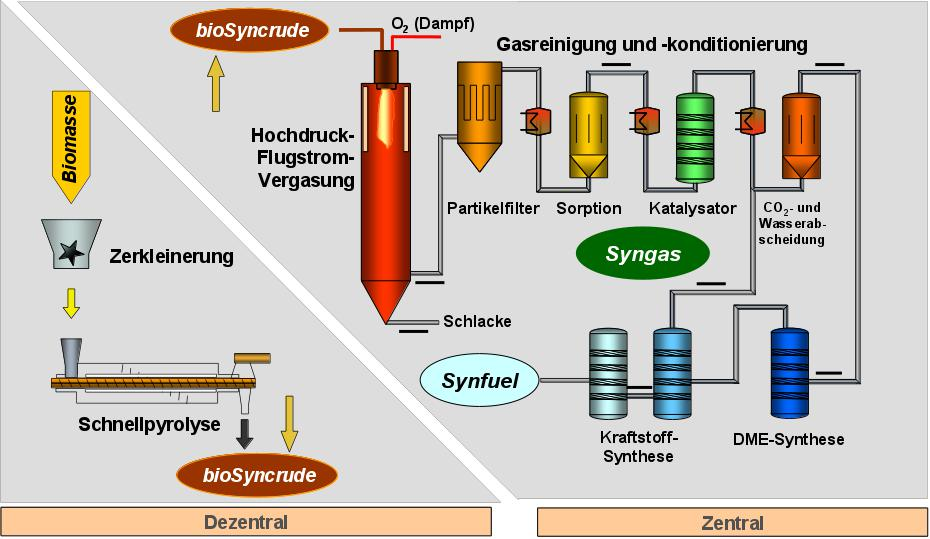
\includegraphics[width=8cm]{material/sebastian/img1.png}
 	} 
 	&
 	\url{https://www.bioliq.de/112.php}
 	\\
 	\vspace*{-1.25\baselineskip}\subsubsection{Conclusion}
 	& 
 	All these processes provide a viable alternative for conventional fuel. But considering, that the aim is to decrease the pollutant emissions and save the earth’s resources CTL fuel and GTL fuel aren't the best options. A better alternative is the production of DME or PODE with biogas. Biogas is obtained from renewable resources and therefore it's more reliable in the long term. 
 	But every option still costs more than the conventional method, which can only be changed by more research for better catalyst and more companies, which try and produce these synthetic fuels.
 	&
 	\\
 	\vspace*{-1.25\baselineskip}\subsubsection{Recommendation}
 	& 
 	At the moment, it's the best option to concentrate the development on BTL fuels like DME or PODE, because those have the biggest positive effect on the environment.
 	&
 	\\
 	\vspace*{-1.25\baselineskip}\subsubsection{Personal Comments}
 	& 
 	It was hard for me to understand how the layout should be and try to adapt my writing style to a not so academic style.
 	&
 	\\
 	\hline
 \end{xtabular}
\newpage
\subsection{Engine Control (Marvin)}
\begin{xtabular}{|p{3.8cm}|p{8.3cm}|p{4.2cm}|}
	%heading
	\vspace*{-1.25\baselineskip}
	\subsubsection{Introduction}
	&
	%main
	The engine control is a vital component of an internal combustion engine (IEC). Today the control of engines in small engines found in cars and trucks is done electrically with a so called \textit{engine control unit} (ECU).
	
	The ECU handles multiple control loops with each fulfilling a specific task. For example:
	& 
	%ref
	\fullcite{kiencke2005}
	\\
	%heading
	&
	%main
	\begin{itemize}
		\item \textbf{Lambda Control}: Controls air/fuel mixture
		\item \textbf{Idle Speed Control}: Keeps the idle speed constant
		\item \textbf{Knock Control}: Prevents knocking
		\item \textbf{Cylinder Balancing}: Ensures smooth running of the engine
	\end{itemize}
	&
	%ref
	\\
	%heading
	\vspace*{-1.25\baselineskip}
	\subsubsection{Findings}
	&
	%main
	For many years, the requirements for an ECU have been pretty much the same. The ECU just had to perform the tasks listed above reliably. Parameters of the engine with its peripherals (which form a dynamic system in sense of control engineering) were constant, i.e. they were assumed to stay at a constant value over time. 
	&
	%ref
	
	\\
	%heading
	Lambda Control
	&
	%main
	On main ECU task is lambda control. With the AFR (air-fuel ratio) controller, the injection of fuel is controlled such that the fuel is burned completely. This helps conserving fuel and is necessary for the so called catalytic converter, which clears the exhaust gases from many pollutants.
	
	This process is illustrated by the following block diagram:
	&
	%ref
	
	\\
	%heading
	
	&
	%main
	{
		\center
		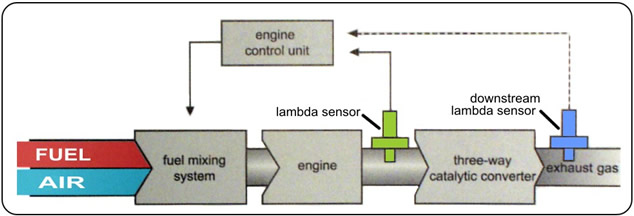
\includegraphics[width=8cm]{material/marvin/LambdaFunctionalDiagram.jpg}
	}
	&
	%ref
	\url{secure.lambdapower.co.uk}
	\\
	%heading
	(Idle) speed control
	&
	%main
	If the car is in neutral, that is no gear is engaged, a constant engine speed (the idle speed) is desired. This is necessary to keep the motor running and to drive auxiliary devices (air conditioning, power steering, ...) In the most cases it is sufficient to control the speed in a quite large band, i.e. in a way that the engine doesn't stall (lower boundary) but doesn't run to fast to conserve fuel and to save the environment (upper boundary).
	
	Constant load situations is another state which should be considered when designing a engine speed controller. Constant load occurs e.g. when driving (without accelerating) on a long flat highway or pulling a trailer up a hill with constant speed. In either case, small speed deviations are tolerable from a technical standpoint.
	&
	%ref
	\fullcite{Subramanian2018}
	\\
	%heading
	\vspace*{-1.25\baselineskip}
	\subsubsection{Problems encountered}
	&
	%main
	In recent years, customers begun to require higher levels of comfort when driving a car or truck. They expect a continual smooth ride regardless of the fuel used and of the usage of additional car accessories.
	&
	%ref
	
	\\
	%heading
	From a consumer point of view
	&
	%main
	Especially modern air conditioning or infotainment systems require much electrical power. To generate the power consumed by these devices, the engine has to drive an alternator. Because these systems can be switched on or off rapidly, they introduce high frequency disturbances to the engine load which the ECU has to remedy. A sophisticated control structure is required in order to prevent high fluctuations of the engine speed which can cause noticeable depreciations of ride smoothness.
	
	Today fossil fuels become more expensive which causes customers to consider fuel ratings when buying a new car. But also the majority of the customers don't want to get to technical with the car. A simple gas stop should be enough.
	&
	%ref
	
	\\
	%heading
	From an environmental point of view
	&
	%main
	In the past, when designing an ECU for an \textsc{Otto} or \textsc{Diesel} engine, the engineer mostly knew what to expect. E.g. gas refined in refineries has very similar properties around the world. Because of that, characteristic curves could be linearized around some operating point. This simplifies analysis and synthesis of control systems dramatically but is only allowed, when the deviations from the operating point are small. If these deviations are large or the operating point is not constant, these simplifications are no more valid and non linear models have to be used.
	
	But to acquire these models, some parameters of the fuel have to be measured (these could include the octane number in the case of gas or the cetan number in the case of diesel). Since it is expensive to measure them and not reasonable to determine them online in the car, they have to be estimated in real time.
	
	This step is rather challenging but vital to ensure emissions complying with the law and to achieve high fuel efficiency ratings.
	&
	%ref
	\\
	%heading
	From the manufactures point of view
	&
	%main
	For the manufacturer it is rather risky to focus on one bio fuel solution at the moment. The car market is volatile and innovations can become successful or die rather quickly. From an engineering and economical perspective, a new ECU should be easily adaptable to different fuel types and optimally completely different technologies.
	&
	%ref
	
	\\
	\vspace*{-1.25\baselineskip}\subsubsection{Solutions}
	& 
	Ideally an ECU lineup would offer an ECU for 'liquid fuel for gas engines' which then automatically adapts to the type of fuel present in the gas tank, without the user noticing.
	&
	\\
	\vspace*{-1.25\baselineskip}\subsubsection{Current Developments}
	& 
	Modern approaches like cascading control or prediction of system states with \textsc{Kalman} filtering could be useful tools when designing a controller.
	&
	\url{https://www.controleng.com/articles/fundamentals-of-cascade-control/}
	\url{http://web.mit.edu/kirtley/kirtley/binlustuff/literature/control/Kalman%20filter.pdf}
		\\
		\vspace*{-1.25\baselineskip}\subsubsection{Conclusion}
		& 
		New ECUs should adapt more modern approaches in control design to allow the usage of new bio fuels.
		&
		\\
		\vspace*{-1.25\baselineskip}\subsubsection{Personal Comments}
		& 
		Research engine control fundamentals specific to new (synthetic) fuels is a quite hard task. Compared to the about 100 years of automobile history, fuels other than gas or diesel are rather new areas of wide scientific interest. Furthermore the development of ECUs in hard- and software is a labour intensive progress mostly done by private companies, which leads to sparse public available information about their inner workings.
		&
		\url{www.bosch-mobility-solutions.com/en/products-and-services/commercial-vehicles/powertrain-systems/natural-gas/electronic-engine-control-unit/}
		\\
		\hline
	\end{xtabular} 

\newpage

\section{Analysis Summaries}
 

\newpage

\section{Resources}
\subsection{Personnel Qualifications List}
\subsubsection{Jakob Heckel}
 
\begin{enumerate}[label=\Alph*.]
	\item \underline{Education}
	
	\begin{tabulary}{\textwidth}{@{}p{3.8cm} C L}
		Since Apr 2019 & - & Karlsruhe Institute of Technology (KIT) \\
		& & Bioengineering Master Studies \\
		\\[-0.5em]
		2015 - 2019 & - & Karlsruhe Institute of Technology (KIT) \\
		& & B.Sc. Bioengineering \\
		\\[-0.5em]
		2012 - 2015 & - & Hochschule für Musik Würzburg (Conservatory) \\
		& & Music/Math teacher training \\
		\\[-0.5em]
		2010 - 2012 & - & Berufsfachschule für Musik Bad Königshofen \\
		& & Conductor for choir and orchestra (classical) \\
		\\[-0.5em]
		2000 - 2010 & - & Secondary Education \\
		& & Gymnasium Scheinfeld \\
	\end{tabulary}
	
	\item \underline{Work Experience}
	
	\begin{tabulary}{\textwidth}{@{}p{3.8cm}CL}
		May 2018 - Oct 2018 & - & Lab Assistant at IFG (@KIT) \\
		& & Produced and assured quality of micro‑thermoformed \newline microcavity-arrays for 3D‑cellculturesystems\\
		\\[-0.5em]
		Dec 2014 - Feb 2015 & - & Harvest worker in Australia \\
		& & Picked lemons, cherries and melons  \\
		\\[-0.5em]
		Oct 2013 - Oct 2914 & - & Minijob at ALDI Süd \\
		& & Placed goods in shelves and assisted customers  \\
	\end{tabulary}
	
	\pagebreak
	\item \underline{Special Skills \& Awards}
	
	\begin{tabulary}{\textwidth}{@{}p{3.8cm}CL}
		Apr 2015 & - & Best-Poster-Award \newline \textit{Comparison of HEP G2-cells in 2D- and 3D-cultivation}\\
		\\[-0.5em]
		& - & Language Skills:           \\
		& & German:  Native Speaker      \\
		& & English: C1 - Proficient     \\
		& & French:  B1 - Independent    \\
		& & Tok Pisin - Melanesian Pidgin\\
		\\[-0.5em]
		
	\end{tabulary}
	
\end{enumerate}

\newpage
\subsubsection{Marvin Noll}
 
\begin{enumerate}[label=\Alph*.]
	\item \underline{Education}
	
	\begin{tabulary}{\textwidth}{@{}p{3.8cm} C L}
		Since Oct 2018 & - & Karlsruhe Institute of Technology (KIT) \\
		& & Electrical Engineering Master Studies - Signal Processing \\
		\\[-0.5em]
		Feb 2016 - Sep 2018 & - & Karlsruhe Institute of Technology (KIT) \\
		& & B. Sc. Electrical Engineering \\
		\\[-0.5em]
		Sep 2012 - Feb 2016 & - & Aalen University (University of Applied Sciences) \\
		& & B. Eng. Optical Engineering \\
		\\[-0.5em]
		2009 - 2012 & - & Secondary Education (A-levels) \\
		& & Berufliche Schulen Korbach und Bad Arolsen \\
	\end{tabulary}
	
	\item \underline{Work Experience}
	
	\begin{tabulary}{\textwidth}{@{}p{3.8cm}CL}
		Since May 2017 & - & Institute of Power Transmission and High Voltage (@ KIT) \\
		& & Lab assistant: \textit{Storing and displaying data of a weather station}\\
		\\[-0.5em]
		May 2018 - Aug 2018 & - & Bruker BioSpin GmbH (Rheinstetten) \\
		& & Internship: \textit{Python GUI for prototype testing; MRI simulations}  \\
		\\[-0.5em]
		May 2017 - Feb 2018 & - & Light Technology Institute (@ KIT) \\
		& & Lab assistant: \textit{Setup a system for radiometric measurements of light bulbs}  \\
		\\[-0.5em]
		Sep 2014 - Feb 2015 & - & Carl Zeiss Meditec AG (Oberkochen) \\
		& & Internship: \textit{Radiometric measurements and fiber optics assessment}  \\
	\end{tabulary}
	
	\pagebreak
	\item \underline{Special Skills \& Awards}
	
	\begin{tabulary}{\textwidth}{@{}p{3.8cm}CL}
		Nov 2016 & - & Optoelectronics Award (from Aalen University for best bachelor thesis)\\
		\\[-0.5em]
		& - & Programming experience: \textit{Python, LabVIEW, MATLAB}\\
		\\[-0.5em]
		& - & CAD: \textit{SolidWorks}\\
		\\[-0.5em]
		& - & Language Skills: \\
		& & German: Native Speaker\\
		& & English: C1 - Proficient \\
		\\[-0.5em]
		
	\end{tabulary}
	
\end{enumerate}

\newpage
\subsubsection{Sebastian Grewe}
 
\begin{enumerate}[label=\Alph*.]
	\item \underline{Education}
	
	\begin{tabulary}{\textwidth}{@{}p{3.8cm} C L}
		Since Oct 2015 & - & Karlsruhe Institute of Technology (KIT) \\
		& & Major - Chemical Engineering - Bachelor Studies \\
		\\[-0.5em]
		2007 - 2015 & - & Secondary Education (A-levels) \\
		& & Ludwig-Marum-Gymnasium, Pfinztal \\
	\end{tabulary}
	
	\item \underline{Work Experience}
	
	\begin{tabulary}{\textwidth}{@{}p{3.8cm}CL}
		Jan 2013 & - & Internship at MiRO (Mineraloelraffinerie Oberrhein) \\
		& & \textit{Working with a reliability engineer. Understanding large \newline industrial plants. Investigating the cause of material malfunction}\\
	\end{tabulary}
	
	\item \underline{Special Skills \& Awards}
	
	\begin{tabulary}{\textwidth}{@{}p{3.8cm}CL}
		Awards & - & Award for the best student in chemistry in secondary Education\\
		\\[-0.5em]
		& - & Language Skills: \\
		& & German:  Native Speaker\\
		& & English: C1 - Proficient \\
		& & French:  B1 - Independent \\
		\\[-0.5em]
		
	\end{tabulary}
	
\end{enumerate}

\newpage

\section{Glossary}
\begin{tabularx}{\textwidth}{p{3cm} l}
	IEC & Internal Combustion Engine \\
	ECU & Engine Control Unit \\
\end{tabularx}	
\newpage

\section{Evaluations}
 

\newpage

\section{Reference List}
\renewcommand{\refname}{Bibliography}
\printbibliography
\newpage

\section{Other}
\subsection{Project Progress}
\begin{ganttchart}{1}{26}
	\gantttitle{CW 26 (June)}{7} \gantttitle{CW 27 (July)}{7} \gantttitle{CW 28 (July)}{7} \gantttitle{CW 29 (July)}{5} \\
	\gantttitlelist{24,...,30}{1} \gantttitlelist{1,...,7}{1} \gantttitlelist{8,...,14}{1} \gantttitlelist{15,...,19}{1} \\
	\ganttgroup{Project Paper}{2}{22} \\
	\ganttbar[bar/.append style={fill=gray!50}]{WP: syngas}{2}{14} \\
	\ganttbar[bar/.append style={fill=green!50}]{WP: synfuel}{3}{16} \\
	\ganttbar[bar/.append style={fill=blue!50}]{WP: engine mod}{3}{15} \\
	\ganttbar[bar/.append style={fill=gray!50}]{Project Statement}{10}{12} \\
	\ganttbar[bar/.append style={fill=green!50}]{Evaluations}{16}{18} \\
	\ganttbar[bar/.append style={fill=gray!50}]{Executive Summary}{17}{18} \\
	\ganttbar[bar/.append style={fill=green!50}]{Analysis Summary}{17}{18} \\
	\ganttbar[bar/.append style={fill=white}]{Proof read}{20}{21} \\
	\ganttmilestone{Finalize Paper}{22} \\
	
	\ganttgroup{Presentation}{14}{21} \\
	\ganttbar[bar/.append style={fill=blue!50}]{Rough structure}{14}{14} \\
	\ganttbar[bar/.append style={fill=green!50}]{Fill slides}{15}{18} \\
	\ganttbar[bar/.append style={fill=white}]{Proof read}{20}{21} \\
	\ganttmilestone{Finalize ppt}{22} \\
	
	\ganttmilestone{Project Due}{24}
	\ganttlink{elem8}{elem9}
	\ganttlink{elem13}{elem14}
	\ganttlink{elem9}{elem15}
	\ganttlink{elem14}{elem15}
	
	\node (a) [fill=gray!50,draw,anchor=west, minimum width=4cm] at ([xshift=91pt, yshift=-20pt] current bounding box.south west)
	{Jakob};
	\node (b) [fill=blue!50,draw,anchor=west, minimum width=4cm] at ([xshift=5pt]a.east)
	{Marvin};
	\node (c) [fill=green!50,draw,anchor=west, minimum width=4cm] at ([xshift=5pt]b.east)
	{Sebastian};
\end{ganttchart}
\newpage

\subsection{Slides of Final Presentation}
\includepdf[pages=-, nup=2x2,landscape=true, delta=12mm 12mm, scale=.7,pagecommand={\pagestyle{fancy}}]{parts/ppt/EE_v2.pdf}

\end{document}